\section{Easy CrackMe}
\begin{enumerate}
\item 运行程序,随意输入,弹窗提示:“Incorrect Password”。\\
\item IDA打开查看函数列表确认没有加壳,直接静态分析。\\
\item
	\begin{enumerate}
	\item Shift + F12  打开Strings窗口,找到字符串“Incorrect Password”,\\
	\item 双击 转到字符串定义,\\
	\item 双击 交叉引用(DATA XREF)的函数名,跳转到对应函数定义,\\
	\item 空格 切换为Graph View分析函数功能 \\
	\end{enumerate} 
\item 
	分析可以弹出消息框“Congratulation !!”的分支(红色箭头):\\
	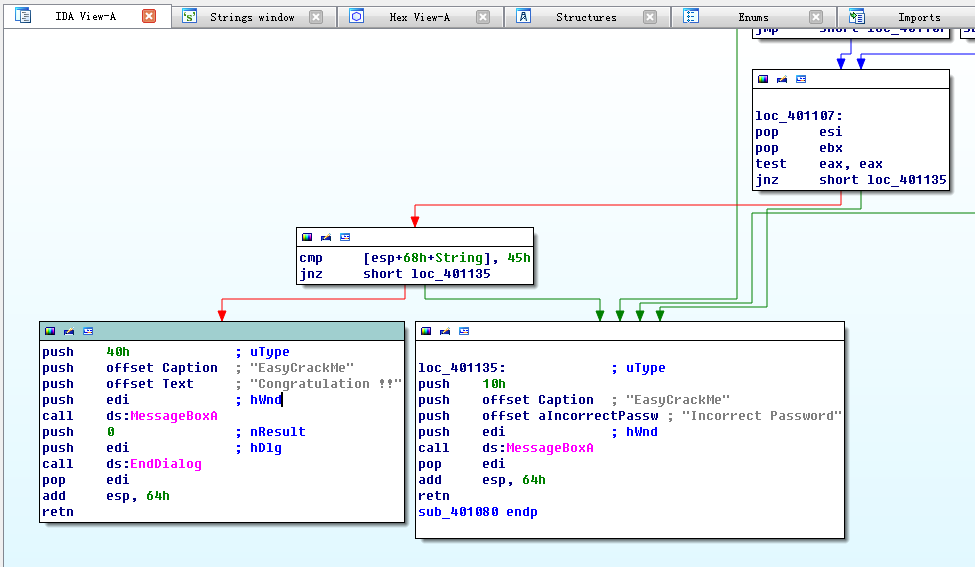
\includegraphics[width=10cm]{easycrack-msgbox.png} \\
	\lstinline$[esp+68h+String]$期望值为E(45h是字符E的ASCII值)
	\begin{lstlisting}
	cmp     [esp+68h+String], 45h
	jnz     short loc_401135
	\end{lstlisting}
	往上查找输入数据,分析GetDlgItemTextA获取输入存放地址:\\
	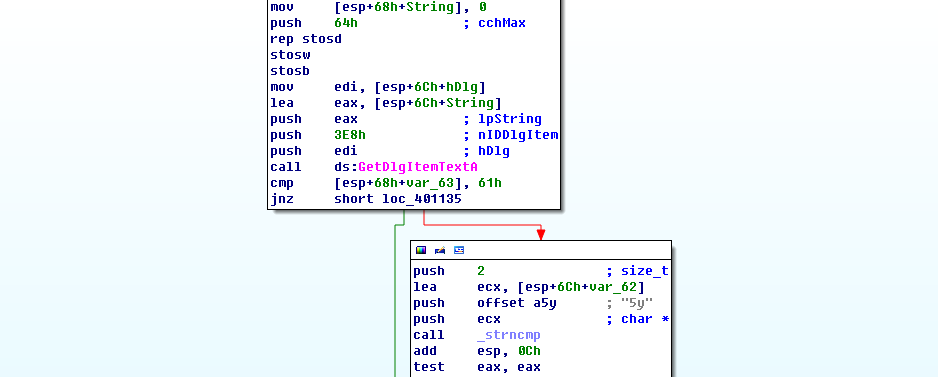
\includegraphics[width=10cm]{easycrack-input.png} \\
	\lstinline$[esp+68h+String]$为存放输入的地址(注意:\lstinline$push    64h    ; cchMax$影响esp的值)
	\begin{lstlisting}
	lea     eax, [esp+6Ch+String]
	push    eax             ; lpString
	\end{lstlisting}
	继续分析,比较输入和期望值
	第一步:\lstinline$[esp+68h+var_63]$期望值为a(61h是字符a的ASCII值)
	\begin{lstlisting}
	cmp     [esp+68h+var_63], 61h
	jnz     short loc_401135
	\end{lstlisting}
	第二步:\lstinline$ [esp+6Ch+var_62]$期望值为“5y”(注意:\lstinline$push    2    ; size_t$影响esp的值)
	\begin{lstlisting}
	lea     ecx, [esp+6Ch+var_62]
	push    offset a5y      ; "5y"
	push    ecx             ; char *
	call    _strncmp
	\end{lstlisting}
	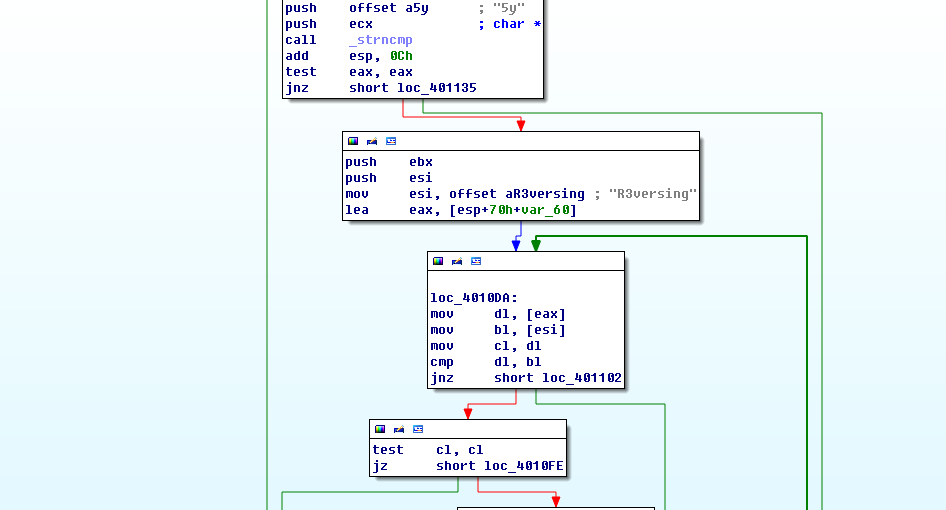
\includegraphics[width=10cm]{easycrack-loop.png} \\
	第三步:\lstinline$[esp+70h+var_60]$期望值为“R3versing”(注意:\lstinline$push ebx$、\lstinline$push esi$影响esp的值)\\
	循环不是很难分析,期望的分支是
	\begin{lstlisting}
	xor     eax, eax
	jmp     short loc_401107
	\end{lstlisting}
	而非
	\begin{lstlisting}
	sbb     eax, eax
	sbb     eax, 0FFFFFFFFh
	\end{lstlisting}
	
	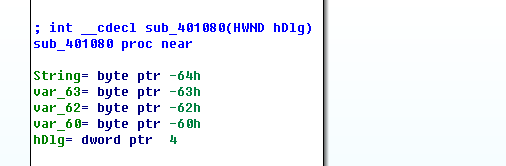
\includegraphics[width=10cm]{easycrack-vars.png} \\
	最后,根据变量定义,将4部分期待字符(串)连接在一起:
	\begin{lstlisting}
	String= byte ptr -64h    ;    `E'
	var_63= byte ptr -63    ;    `a'
	var_62= byte ptr -62h    ;    ``5y''
	var_60= byte ptr -60h    ;    ``R3versing''
	\end{lstlisting}
	flag : ``Ea5yR3versing''
\end{enumerate}